% -*- LaTeX -*-
% -*- coding: utf-8 -*-
%
% michael a.g. aïvázis
% california institute of technology
% (c) 1998-2012 all rights reserved
%

\lecture{Exchanging data with MPI}{20120201}

% --------------------------------------
% sending and receiving messages
\begin{frame}[fragile]
%
  \frametitle{Point to point communication}
%
  \begin{itemize}
%
  \item to send a message
    \begin{C}
int MPI_Send(
        void* buffer, int count, MPI_Datatype datatype,
        int destination, int tag, MPI_Comm communicator
        );
   \end{C}
%
  \item to receive a message
    \begin{C}
int MPI_Recv(
        void* buffer, int count, MPI_Datatype datatype,
        int source, int tag, MPI_Comm communicator
        );
   \end{C}
%
  \item the \identifier{tag} enables choosing the order you may receive pending messages
%
  \item but for a given (\identifier{source},\identifier{tag},\identifier{communicator})
    messages are received in the order they were sent
%
  \item receiving via wildcards: \identifier{MPI\_ANY\_SOURCE} and \identifier{MPI\_ANY\_TAG}
% 
  \item in {\em standard} communication mode, sending and receiving messages are {\em blocking},
   so the function does not return until you can safely access the \identifier{buffer}
   \begin{itemize}
   \item to read, free, etc.
   \end{itemize}
%
  \end{itemize}
%
\end{frame}

% --------------------------------------
% communication modes
\begin{frame}[fragile]
%
  \frametitle{Communication modes}
%
  \begin{itemize}
%
  \item in standard mode, the specification does not explicitly mention buffering strategy
    \begin{itemize}
    \item buffering messages would remove some of the access constraints but it requires time
      and storage for the multiple copies
    \item portability across implementations implies conservative assumptions about the order
      of initiation of sends and receives to avoid deadlock
    \end{itemize}
%
  \item in {\em ready} mode, you must post a receive before the matching send can be initiated
    \begin{itemize}
    \item \function{MPI\_Rsend}, \function{MPI\_Rrecv}
    \end{itemize}
%
  \item in {\em buffered} mode, sends can be initiated, and may complete, regardless of when
    the matching receive is initiate
    \begin{itemize}
    \item \function{MPI\_Bsend}, \function{MPI\_Brecv}
    \end{itemize}
%
  \item in {\em synchronous} mode, sends can be initiated regardless of whether the matching
    receive has been initiated, but the send will not return until the message has been
    received
    \begin{itemize}
    \item \function{MPI\_Ssend}, \function{MPI\_Srecv}
    \end{itemize}
  \end{itemize}
%
\end{frame}

% --------------------------------------
% asynchronous communications
\begin{frame}[fragile]
%
  \frametitle{Asynchronous communication}
%
  \begin{itemize}
%
  \item there are non-blocking versions of all these
    \begin{C}
int MPI_Isend(
        void* buffer, int count, MPI_Datatype datatype,
        int destination, int tag, 
        MPI_Comm communicator, MPI_Request* request
        );
    \end{C}
    \begin{itemize}
    \item faster, but you must take care to not access the message buffers until the messages
      have been delivered
    \item more details later in the course, as needed
    \end{itemize}
%
  \item for sends
    \begin{itemize}
    \item standard mode: \function{MPI\_Isend}
    \item ready mode: \function{MPI\_Irsend}
    \item buffered mode: \function{MPI\_Ibsend}
    \item synchronous mode: \function{MPI\_Issend}
    \end{itemize}
%
  \item only one call for receives: \function{MPI\_Irecv}
%
  \item extra \identifier{request} argument to check for completion of the request
    \begin{itemize}
    \item \function{MPI\_Test}, \function{MPI\_Wait} and their relatives
    \end{itemize}
%
  \end{itemize}
%
\end{frame}

% --------------------------------------
% creating communicators and groups
\begin{frame}[fragile]
%
  \frametitle{Creating communicators and groups}
%
  \begin{itemize}
%
  \item communicators and groups are intertwined  
    \begin{itemize}
    \item you cannot create a group without a communicator
    \item you cannot create a communicator without a group
    \end{itemize}
%
  \item the cycle is broken by \identifier{MPI\_COMM\_WORLD}
    \begin{C}[basicstyle=\tt\bfseries\tiny]
#include <mpi.h>

int main(int argc, char* argv[]) {
    /* declare a communicator and a couple of groups */
    MPI_Comm workers;
    MPI_Group world_grp, workers_grp;

    /* initialize MPI; for brevity all status checks are omitted */
    MPI_Init(&argc, &argv);

    /* get the world communicator to build its group */
    MPI_Comm_group(MPI_COMM_WORLD, &world_grp);

    /* build another group by excluding a process */
    MPI_Group_excl(world_grp, 1, 0, &workers_grp);

    /* now build a communicator out of the processes in workers_grp */
    MPI_Comm_create(MPI_COMM_WORLD, worker_grp, &workers);

    /* etc.... */

    /* shut down MPI */
    MPI_Finalize();

    return 0;
}
    \end{C}
%
  \end{itemize}
%
\end{frame}

% --------------------------------------
% freeing communicators and groups
\begin{frame}[fragile]
%
  \frametitle{Manipulating communicators and groups}
%
  \begin{itemize}
%
  \item releasing resources
    \begin{C}
int MPI_Group_free(MPI_Group* group);
int MPI_Comm_free(MPI_Comm* communicator);
int MPI_Comm_disconnect(MPI_Comm* communicator);
    \end{C}
%
  \item you can make a new group by adding or removing processes from an existing one
    \begin{C}
int MPI_Group_incl(
    MPI_Group grp, int n, int* ranks, MPI_Group* new_group);
int MPI_Group_excl(
    MPI_Group grp, int n, int* ranks, MPI_Group* new_group);
    \end{C}
%
  \item or by using set operations
    \begin{C}
int MPI_Group_union(
    MPI_Group grp1, MPI_Group grp2, MPI_Group* new_group);
int MPI_Group_intersection(
    MPI_Group grp1, MPI_Group grp2, MPI_Group* new_group);
int MPI_Group_difference(
    MPI_Group grp1, MPI_Group grp2, MPI_Group* new_group);
    \end{C}
%
  \end{itemize}
%
\end{frame}

% --------------------------------------
% timing
\begin{frame}[fragile]
%
  \frametitle{Timing}
%
  \begin{itemize}
%
  \item the function
    \begin{C}
double MPI_Wtime();
    \end{C}
    returns the time in seconds from some arbitrary time in the past
    \begin{itemize}
    \item guaranteed not to change only for the duration of the process
    \end{itemize}
%
  \item you can compute the elapsed time for any program segment by making calls at the
    beginning and the end and computing the difference
%
  \item no guarantees about synchronized clocks among different processes
%
  \item you can compute the clock resolution by using
    \begin{C}
double MPI_Wtick();
    \end{C}
%
  \end{itemize}
%
\end{frame}

% --------------------------------------
% other collective operations
\begin{frame}[fragile]
%
  \frametitle{Other collective operations}
%
  \begin{itemize}
%
  \item \function{MPI\_Scan} computes partial reductions: the \th{p} process receives the
    result from processes 0 through $p-1$
    \begin{C}
int MPI_Scan(
        void* send_buffer, void* recv_buffer,
        int count, MPI_Datatype datatype, MPI_Op operation,
        MPI_Comm communicator
        );
   \end{C}
%
  \item \function{MPI\_Reduce} collects the result at only the given process \identifier{root}
    \begin{C}
int MPI_Reduce(
        void* send_buffer, void* recv_buffer,
        int count, MPI_Datatype datatype, MPI_Op operation,
        int root, MPI_Comm communicator
        );
   \end{C}
%
   \item synchronization is also a global operation:
    \begin{C}
int MPI_Barrier(MPI_Comm communicator);
   \end{C}
%
   participating processes block at a barrier until they have all reached it
%
  \end{itemize}
%
\end{frame}

% --------------------------------------
% scatter
\begin{frame}[fragile]
%
  \frametitle{Scatter}
%
  \begin{itemize}
%
  \item \function{MPI\_Scatter} sends data from \identifier{root} to all processes 
    \begin{C}
int MPI_Scatter(
        void* send_buffer, int send_count, MPI_Datatype send_datatype,
        void* recv_buffer, int recv_count, MPI_Datatype recv_datatype,
        int root, MPI_Comm communicator
        );
    \end{C}
    \begin{figure}
      \centering
      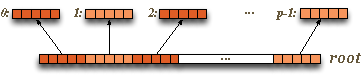
\includegraphics[scale=1.0]{figures/mpi-scatter.pdf}
    \end{figure}
%
  \item it is as if the data in \identifier{send\_buffer} were split in $p$ segments, and the
    \th{i} process receives the \th{i} segment
%
  \item the \identifier{send\_xxx} arguments are only meaningful for \identifier{root}; they
    are ignored for other processes
%
  \item the arguments \identifier{root} and \identifier{communicator} must be passed identical
    values by all processes
%
  \end{itemize}
% 
\end{frame}

% --------------------------------------
% gather
\begin{frame}[fragile]
%
  \frametitle{Gather}
%
  \begin{itemize}
%
  \item the converse is \function{MPI\_Gather} with \identifier{root} receiving data from all
    processes
    \begin{C}
int MPI_Gather(
        void* send_buffer, int send_count, MPI_Datatype send_datatype,
        void* recv_buffer, int recv_count, MPI_Datatype recv_datatype,
        int root, MPI_Comm communicator
        );
   \end{C}
   \begin{figure}
     \centering
     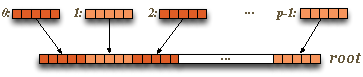
\includegraphics[scale=1.0]{figures/mpi-gather.pdf}
   \end{figure}
%
  \item it is as if $p$ messages, one from each processes, were concatenated in rank order and
    placed at \identifier{recv\_buffer}
%
  \item the \identifier{recv\_xxx} arguments are only meaningful for \identifier{root}; they
    are ignored for other processes
%
  \item the arguments \identifier{root} and \identifier{communicator} must be passed identical
    values by all processes
%
  \end{itemize}
%
\end{frame}

% --------------------------------------
% broadcasts
\begin{frame}[fragile]
%
  \frametitle{Broadcasting operations}
%
  \begin{itemize}
%
  \item \function{MPI\_Alltoall} sends data from all processes to all processes in a global
    scatter/gather
    \begin{C}
int MPI_Alltoall(
        void* send_buffer, int send_count, MPI_Datatype send_datatype,
        void* recv_buffer, int recv_count, MPI_Datatype recv_datatype,
        MPI_Comm communicator
        );
   \end{C}
%
 \item use \function{MPI\_Bcast} to send the contents of a buffer from \identifier{root} to all
   processes in a communicator
   \begin{C}
int MPI_Bcast(
        void* buffer, int count, MPI_Datatype datatype,
        int root, MPI_Comm communicator
        );
   \end{C}
%
  \end{itemize}
%
\end{frame}

% --------------------------------------
% collective operations summary
\begin{frame}[fragile]
%
  \frametitle{Data movement patterns for the collective operations}
%
  \begin{tabular}{cc}
    \parbox[c][1in]{2in}{
      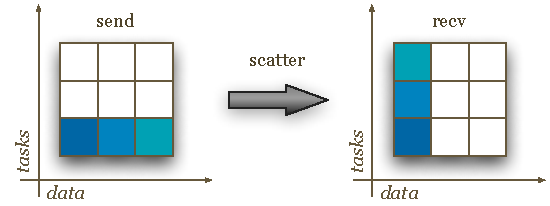
\includegraphics[scale=0.5]{figures/mpi-scatter-pattern.pdf}
    }
    &
    \parbox[c][1in]{2in}{
      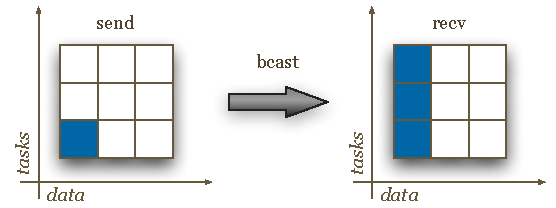
\includegraphics[scale=0.5]{figures/mpi-bcast-pattern.pdf}
    }
    \\ 
    \parbox[c][1in]{2in}{
      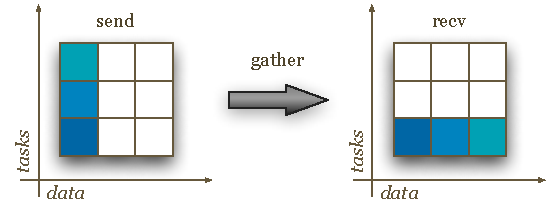
\includegraphics[scale=0.5]{figures/mpi-gather-pattern.pdf}
    }
    &
    \parbox[c][1in]{2in}{
      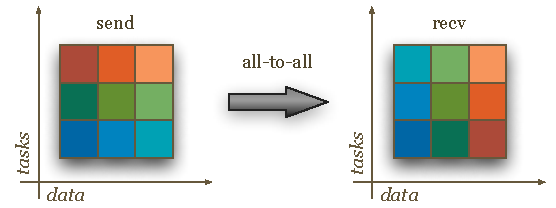
\includegraphics[scale=0.5]{figures/mpi-alltoall-pattern.pdf}
    }
  \end{tabular}
%
\end{frame}

